%Como o avanço da computação foi e é grandioso, é normal e esperado que abranja área que antes ele não alcançava. Então, cada vez mais, o mercado, as pessoas, as empresas necessitam e requisitam softwares com finalidades variadas e assim fazendo com que surgirem vários ramos de desenvolvimento. Então surgiu a necessidade de criação de um padrão de desenvolvimento, para não somente auxiliar como também definir limites e regras para: criação, documentação e manutenção. Assim surgiu a engenharia de software.\\

%Para essa aplicação escolheu-se o modelo de desenvolvimento sequencial ou cascata(Figura~\ref{fg:modelo_dev}), que é uns dos mais antigos e também mais utilizados. 
%\begin{figure}[ht!]
%	\centering
%	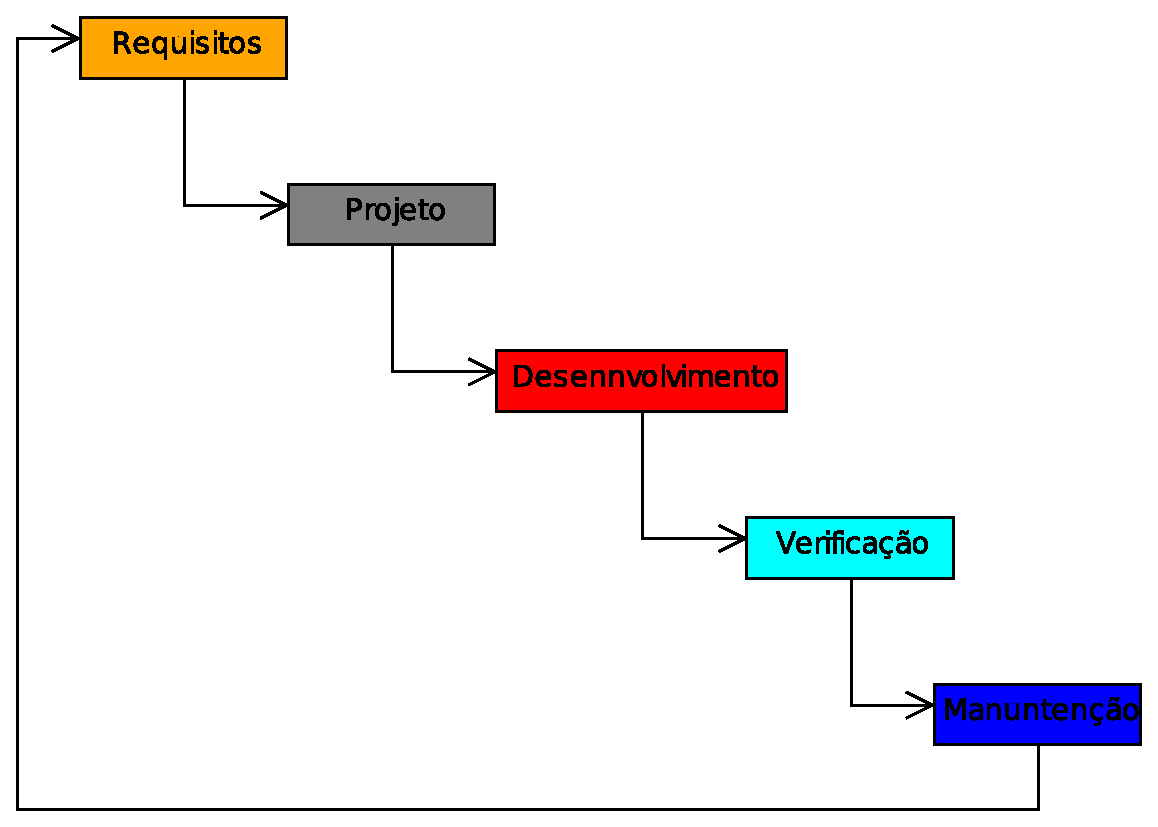
\includegraphics[scale=0.35]{modelo_dev}
%	\caption{Modelo de desenvolvimento cascata.}
%	\label{fg:modelo_dev}
%\end{figure}

	\subsection{Tecnologias de Programação Usadas} 
	As tecnologias de programação usadas foram: o motor gráfico de jogos irrlicht, a plataforma Qt-Creator e a linguagem C++. As informações sobre a engine irrlicht estão na seção $2.2$. O Qt-Creator é um poderoso ambiente multi plataforma que permite a criação de diversas aplicações web e também desktop. O uso dele, neste trabalho, foi voltado para a criação de uma interface desktop, a qual pudesse ser usada em diferentes sistemas operacionais(Linux, Windows ou Macintoch) e com arquiteturas dissemelhante(32 ou 64 bits). Tanto essa plataforma quanto a linguagem foram escolhidas por serem muito usadas pelo comunidade desenvolvedora, por serem robustas e terem uma ótima documentação.
	
	\subsection{Conexão Qt-Irrlicht}
	O primeiro passo no desenvolvimento desse trabalho foi a união do universo irrlicht com a plataforma Qt-Creator. Para tanto foi necessário o estudo das classes e funcionalidades básicas desse dois mundos.\\
	
	A ideia era colocar o motor gráfico irrlicht funcionando como uma janela dentro da interface gerenciada pelo qt. Assim criou-se a classe base de todo esse projeto, chamada IrrViewer. Ela contem os métodos base de uma classe Widget\footnote{Janela padrão do qt.}, que são : paintEvent(), resizeEvent() e paintEngine(); e também os necessários para a criação de um cenário 3D irrlicht, os quais são : createIrrlichtDevice()(reponsável pela criação do \textit{device}\footnote{Responsável por todas as informações da cena}, \textit{smgr}\footnote{Gerenciador de cena, ele que responsável por adicionar, remover, clonar e capturar objetos da cena.} e \textit{video-driver}\footnote{Responsável por tudo referente ao driver de video}), cenaIrrlicht()(método que tem a finalidade de criar a cena), drawIrrlichtScene()(método de pintura).\\
	
	Assim, com o Qt-Creator reconhecendo essa nova classe como uma janela(Widget) normal, pode-se passar para outra fase proposta, que era a criação de outras classes e métodos necessários para concretização do requisitos pré-estabelecidos para esse trabalho.

	\subsection{Classes}
	As classes criadas para este projeto foram: \textit{IrrViewer, Cena, IrrNode, ReceiverEvent} e \textit{MainWindow}. A primeira é a base de todo o desenvolvimento do software produzido nesse projeto, é a que conectar o irrlicht com o Qt. A classe \textit{Cena} contem e controla tudo referente a cena,tal como: seleção, inserção, modificação e deleção de \textit{nós}; Assim como também a geração de malha e eventos de mouse e teclado. A terceira classe é responsável pela criação de objetos: prisma, cubo, esfera, cone, haste, cilindro e antena.\\
	
	Já a classe \textit{ReceiverEvent} tem como finalidade receber os eventos de mouse do Qt e repassá-los para a engine irrlicht. Por fim, temos a classe MainWindow que é a interface em si, onde se encontram os botões e \textit{signals and slots}\cite{qt}.

\section{Interface}
A interface feita nesse projeto esta representada na Figura~\ref{fg:layout}. Ela foi baseada nos softwares de modelagem mais usados no mercado, que são : Blender, 3DStudio e Maya. A sua estrutura foi dividida em 4 áreas: barra superior, janela da cena, painéis laterais e barra inferior.\\

\begin{figure}[ht!]
	\centering
	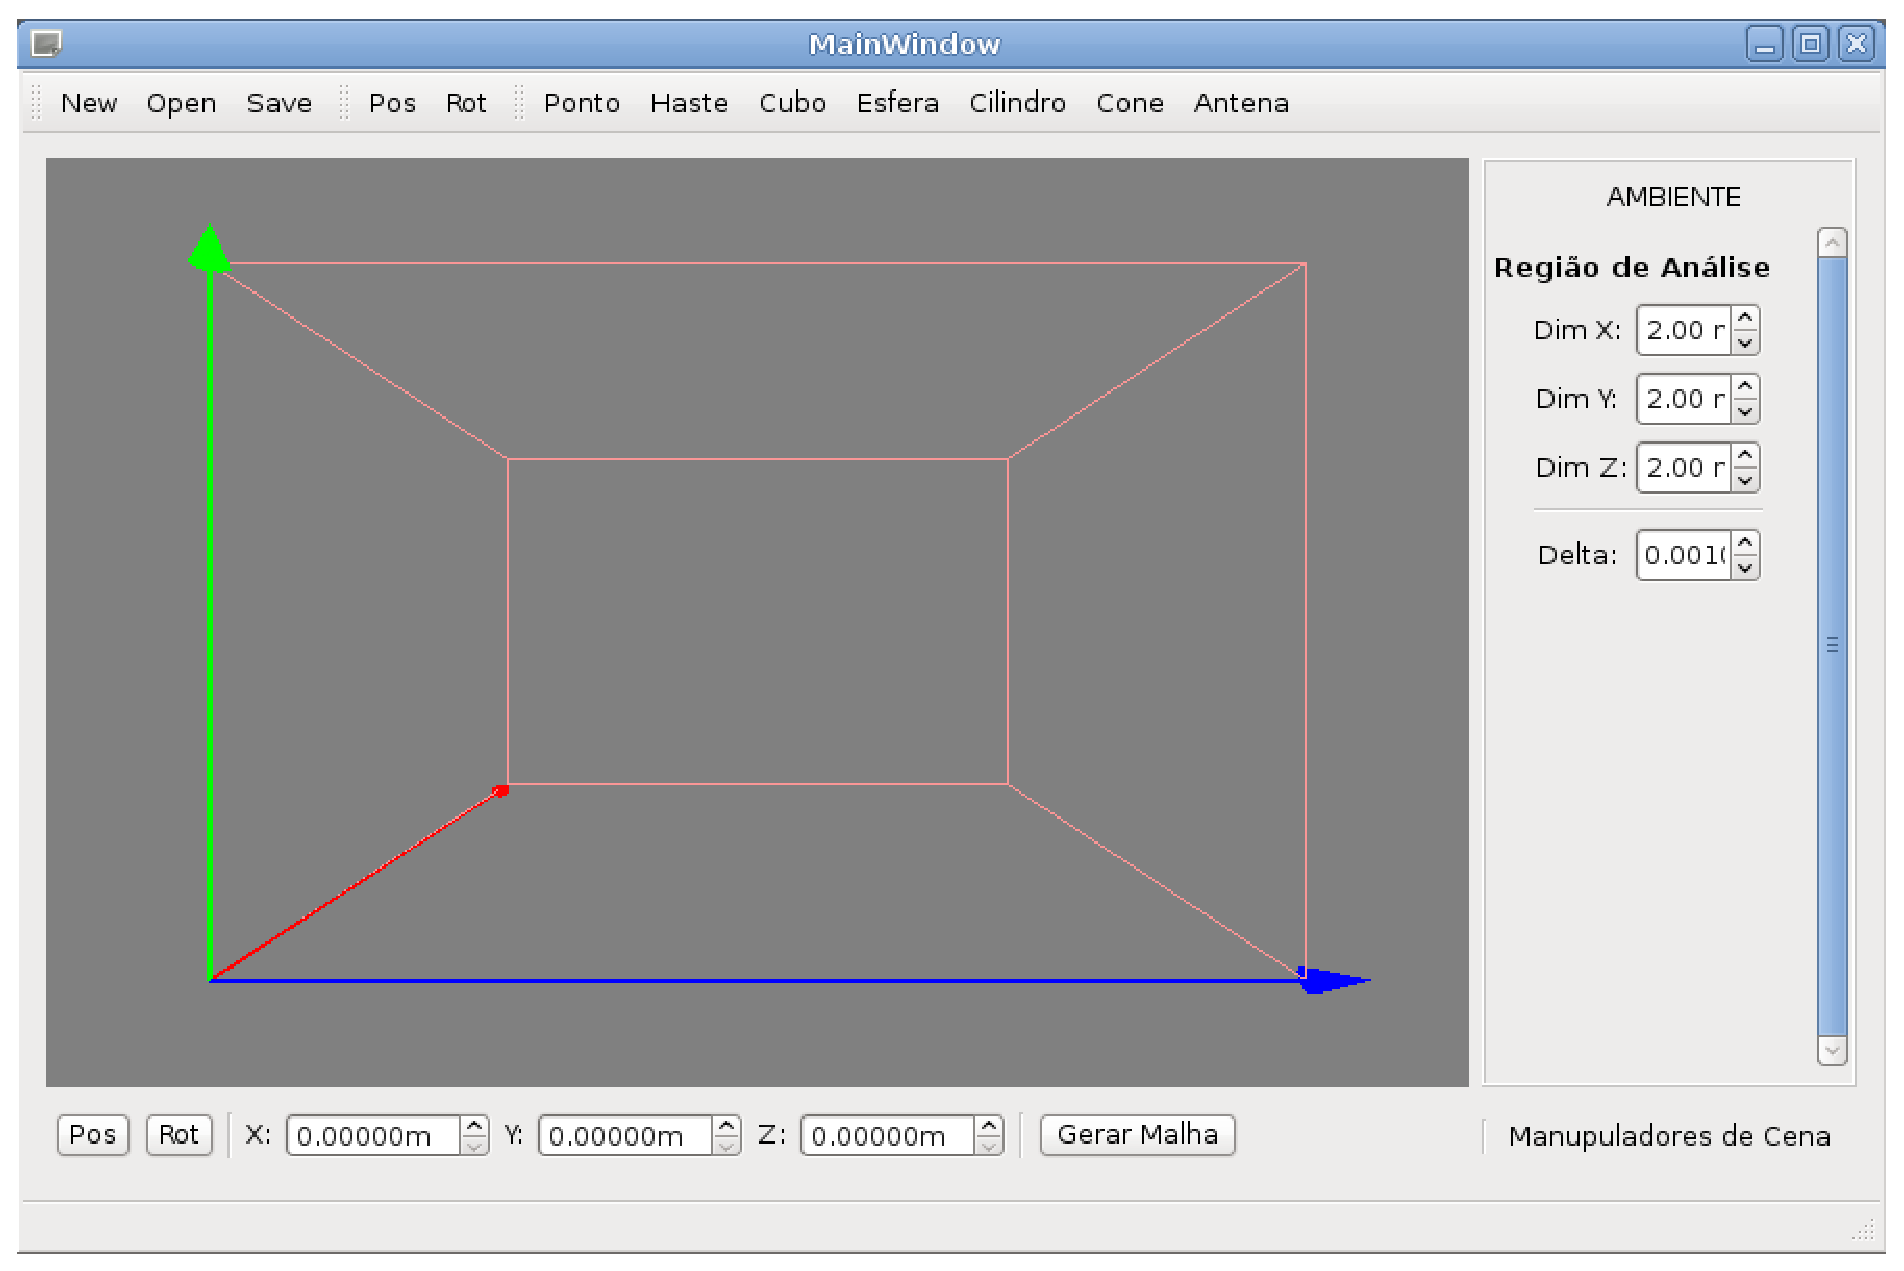
\includegraphics[scale = 0.4]{layout}
	\caption{Layout interface.}
	\label{fg:layout}
\end{figure}

Na barra superior, Figura~\ref{fg:barra_s}, encontramos primeiramente o botão \textit{New}, o qual ativará uma nova cena irrlicht. Quando pressionado ativara uma janela(Figura~\ref{fg:dados_r}) que requisitará os dados necessários para criação da região de análise, tais como dimensão $x$, $y$, $z$ e o valor do $delta$(dimensão da célula de Yee). Em seguida vem o botão \textit{Open}, que carrega uma cena anterior caso tenha já exista alguma salva. Depois dele temos o botão \textit{Save}, que salva a cena atual em uma arquivo chamado \textit{Map.in}, que contem todas as características dos objetos(dimensões, tipo e parâmetros de material) assim como suas posições.\\

\begin{figure}[ht!]
	\centering
	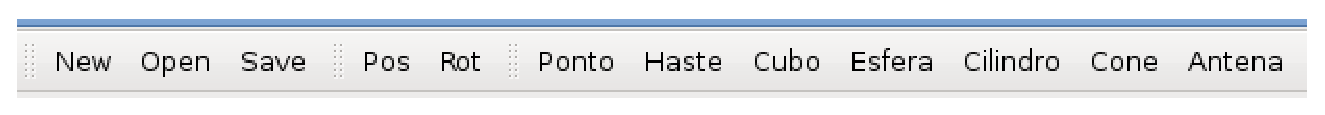
\includegraphics[scale = 0.4]{barra_s}
	\caption{Barra Superior interface.}
	\label{fg:barra_s}
\end{figure}
\begin{figure}[ht!]
	\centering
	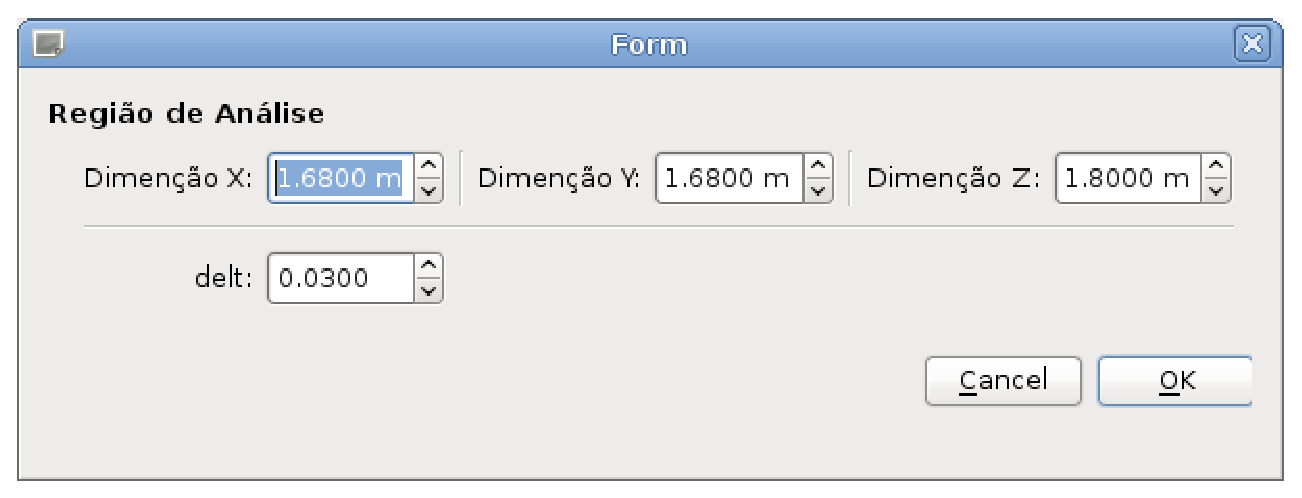
\includegraphics[scale = 0.4]{dados_r}
	\caption{Janela com as caracteristica da região de análise.}
	\label{fg:dados_r}
\end{figure}

Seguindo encontramos os botões \textit{Pos} e \textit{Rot}, os quais quando pressionados mostram o posicionamento e ângulos de rotação dos objetos selecionados respectivamente. Logo em seguida temos os criadores de objetos básico da interface, que são \textit{Ponto},\textit{Haste}, \textit{Cubo}, \textit{Esfera}, \textit{Cilindro}, \textit{Cone} e por fim \textit{Antena}. Quando ativados criam o objeto desejado com os parâmetros especificados, assim como sua posição.\\

A janela da cena, Figura~\ref{fg:janela_c} é onde visualizamos nosso universo virtual. O painel lateral, Figura~\ref{fg:painel_l} é onde encontramos as características como dimensão e parâmetros manterias do objeto selecionado ou criado.\\

\begin{figure}[ht!]
	\centering
	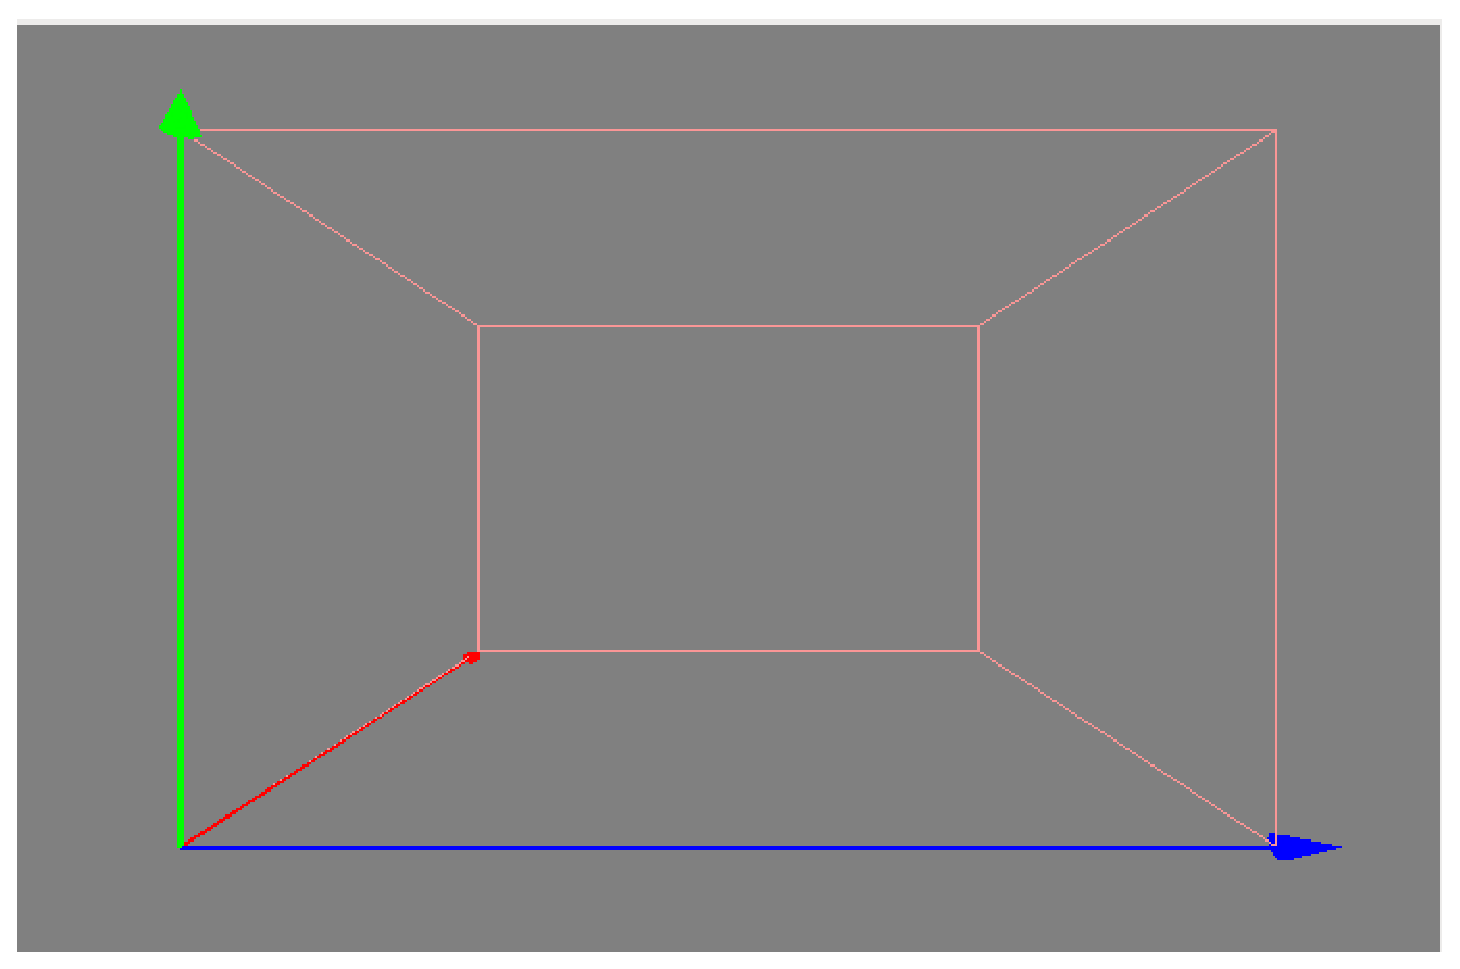
\includegraphics[scale = 0.4]{janela_c}
	\caption{Janela da Cena.}
	\label{fg:janela_c}
\end{figure}
\begin{figure}[ht!]
	\centering
	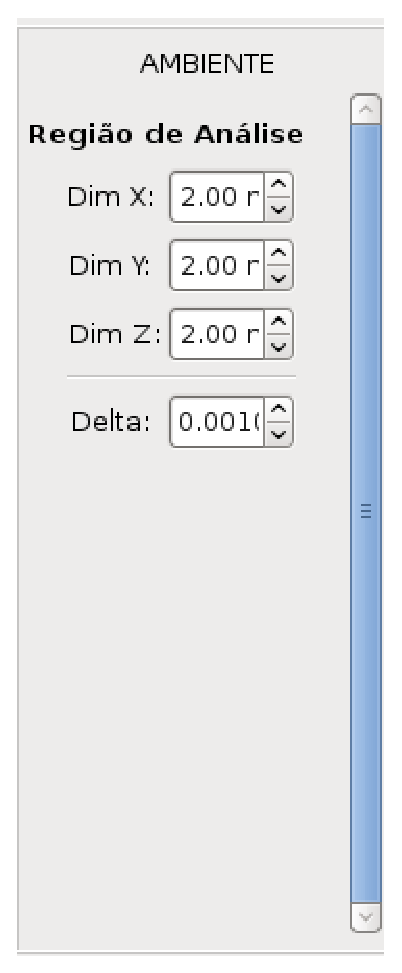
\includegraphics[scale = 0.4]{painel_l}
	\caption{Painel lateral dos parâmetros da região de análise.}
	\label{fg:painel_l}
\end{figure}

Na parte inferior da interface(Figura~\ref{fg:barra_i}) encontram-se os botões \textit{Pos} e \textit{Rot}, que têm as mesmas funcionalidades dos já sitados da barra superior. Assim como a coordenada do objeto selecionado($X$, $Y$ e $Z$). E por fim esta o botão \textit{gerar Malha}, o qual tem a função de gerar a malha compatível com o simulador LANE-SAGS.

\begin{figure}[ht!]
	\centering
	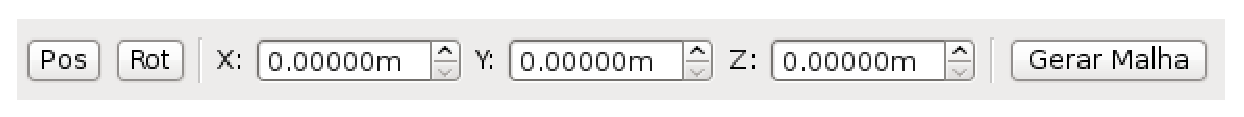
\includegraphics[scale = 0.4]{barra_i}
	\caption{Barra inferior da interface.}
	\label{fg:barra_i}
\end{figure}

\section{Funcionalidades}
	\subsection{Eventos de Mouse e Teclado}
	Tanto o irrlicht quanto o a biblioteca qt têm suporte a eventos de mouse e teclado. Todavia, o evento de mouse é visto e realizado de forma distinta. Então apareceu a necessidade de criação de um tipo de "comunicador" que "traduzisse" esse evento entres esses mundos diferentes.\\
	
	Na interface esse "comunicador" basicamente pegar as informações de mouse da janela do qt e envia de forma traduzida para o motor gráfico irrlicht. São basicamente três métodos do qt que foram modificados: mouseMoveEvent(), mousePressEvent() e mouseReleaseEvent().\\
	
	Já o evento de teclado não foi necessário o uso do "comunicador", pelo fato de não haver necessidade usarmos esse tipo de evento no irrlicht. Foram criados vários atalhos de teclado para facilitar a manipulação e navegação na cena, listados na tabela a seguir:
	
\begin{center}
\begin{tabular}{|l|l|}
    \hline
	Atalho & Funcionalidade \\ \hline
	Shift+O &  Afastamento\\ \hline
	Shift+P &  Aproximação\\ \hline
	W & Focaliza objeto selecionado\\ \hline
	C & Clona objeto selecionado(duplica)\\ \hline
	R & Remove objeto selecionado \\ \hline
	1 & Muda para camera frente \\ \hline
	2 & Muda para camera lateral esquerda \\ \hline
	3 & Muda para camera lateral direita \\ \hline
	4 & Muda para camera traseira \\ \hline
	5 & Muda para camera topo \\ \hline
	6 & Muda para camera base \\ \hline
	M + X & Permite movimentação de objeto selecionado no eixo X com o mouse \\ \hline
	M + Y & Permite movimentação de objeto selecionado no eixo Y com o mouse \\ \hline
	M + Z & Permite movimentação de objeto selecionado no eixo Z com o mouse \\ \hline
	Shift + A & Permite movimentação de objeto selecionado nos eixos X e Y com o mouse \\ \hline
	Shift + B & Permite movimentação de objeto selecionado nos eixos X e Z com o mouse \\ \hline
	Shift + C & Permite movimentação de objeto selecionado nos eixos Y e Z com o mouse \\ \hline
	Shift + D & Permite movimentação de objeto selecionado nos eixos X, Y e Z com o mouse \\ 
    \hline
\end{tabular}
\end{center}
	
	\subsection{Colisão}
	O evento de colisão foi feito baseado na teoria de jogos. Existem vários tipos de colisão, porém a utilizada nesse trabalho foi a de resposta por reta. Seu funcionamento é bem simples, cria-se uma reta imaginária na cena onde seu ponto de origem é a câmera e seu fim esta localizado em um ponto bastante distante ao inicial. Esse ponto final acompanha o movimento do mouse. Então quando clica-se em um dado ponto do universo criado na interface é disparado o evento de colisão o qual retorna {nó}\footnote{Objeto selecionado} selecionado. \\
	
	Mas isso só vale quando o há um objeto na coordenada selecionada sendo ele selecionável. No caso de se clicar em um dos gizmos\footnote{Orientadores de eixo, gizmo verde(representa o eixo $y$), gizmo azul(representa o eixo $x$) e gizmo vermelho(representa o eixo $z$)} da região de análise, por exemplo, o evento de colisão retornará um objeto vázio, apesar de o gizmo ser um objeto normal ele foi configurado como não selecionável assim fazendo com que mesmo que a reta colida com ele o resultado será nulo. A Figura~\ref{fg:colision} mostra a ocorrência desse evento na interface, como pode-se observar o objeto selecionado é pintado na sua forma armada ou wireframe para diferenciar dos não selecionados.
	
\begin{figure}[ht!]
	\centering
	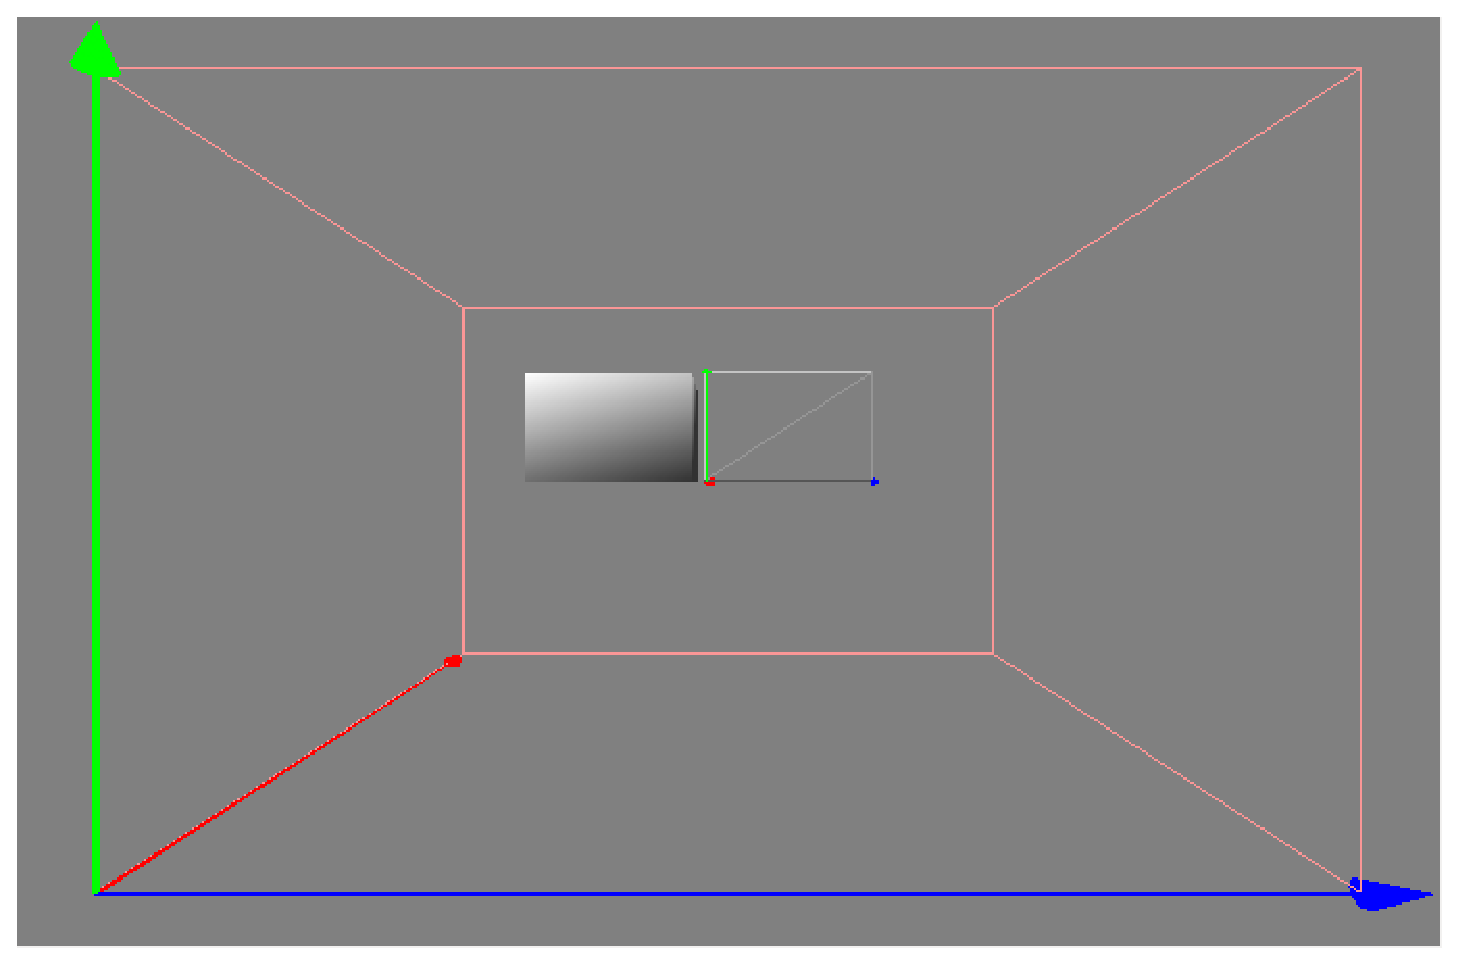
\includegraphics[scale = 0.4]{colision}
	\caption{Ilustração do evento de colisão com o objeto cubo.}
	\label{fg:colision}
\end{figure}

	\subsection{Visualizações}
	Ter vários ângulos de visualização é fundamental quando esta se modelando um ambiente 3D, principalmente quando vamos usá-lo para simulação de ondas eletromagnéticas pelo fato de qualquer erro deixado na estrutura poderá alterar no resultado final. Para sanar esse problema, o software confeccionado nesse projeto, permitir visualizar a região de análise por seis câmeras diferentes: frente(padrão), lateral esquerda, lateral direita, por trás, topo e base. 
	
	\subsection{Aproximação e Afastamento}
	É uma característica importante da interface criada nesse projeto. Ela permite se aproximar(através do atalho de teclado Shift+P) e afastar(por meio de Shift+O) conforme desejarmos de uma objeto que se encontra dentro da região de análise. Assim permitindo navegar pelo cenário virtual criado, podendo alterar, remover e duplicar objetos conforme desejado. Uma outra especificação dessa propriedade esta associada ao fato de quando temos um objeto selecionado. Se pressionarmos a tecla W a câmera ira ter como foco esse objeto. Para melhor entendimento a Figura~\ref{fg:nor} mostra a visualização de um objeto sem alteração de foco da câmera e distancia, já a Figura~\ref{fg:afas} mostra a visualização após um determinado afastamento e por fim as Figuras~\ref{fg:apr} e \ref{fg:w} mostram a aproximação normal e a por seleção.
	
\begin{figure}[ht!]
	\centering
	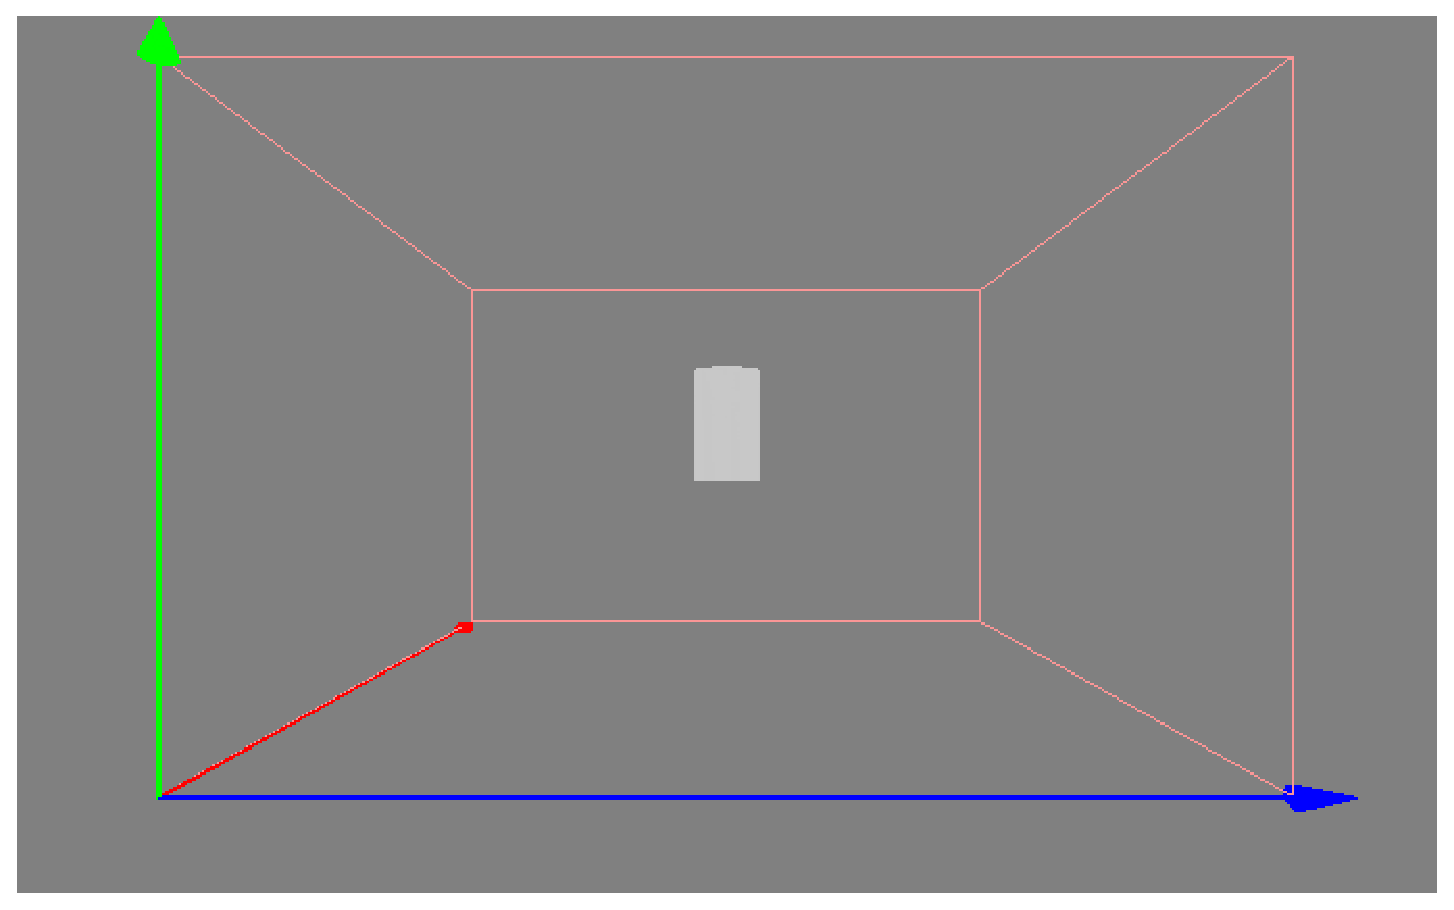
\includegraphics[scale = 0.4]{nor}
	\caption{Visualização de objeto cilindro sem aproximação, afastamento ou mudança de foco da câmera.}
	\label{fg:nor}
\end{figure}
\begin{figure}[ht!]
	\centering
	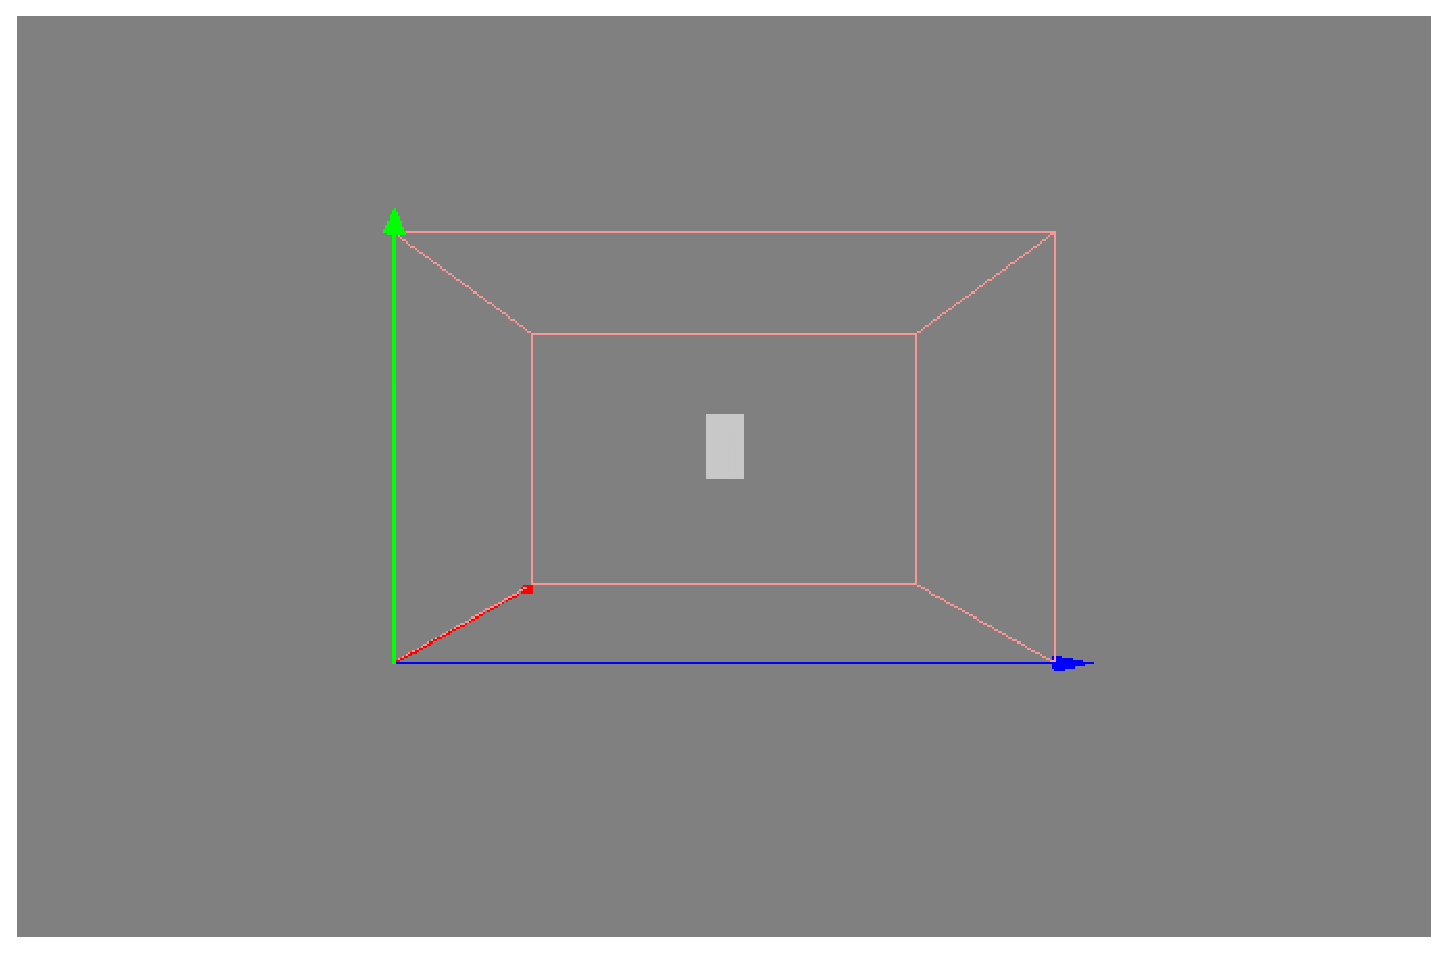
\includegraphics[scale = 0.4]{afas}
	\caption{Visualização de objeto cilindro com afastamento.}
	\label{fg:afas}
\end{figure}
\begin{figure}[ht!]
	\centering
	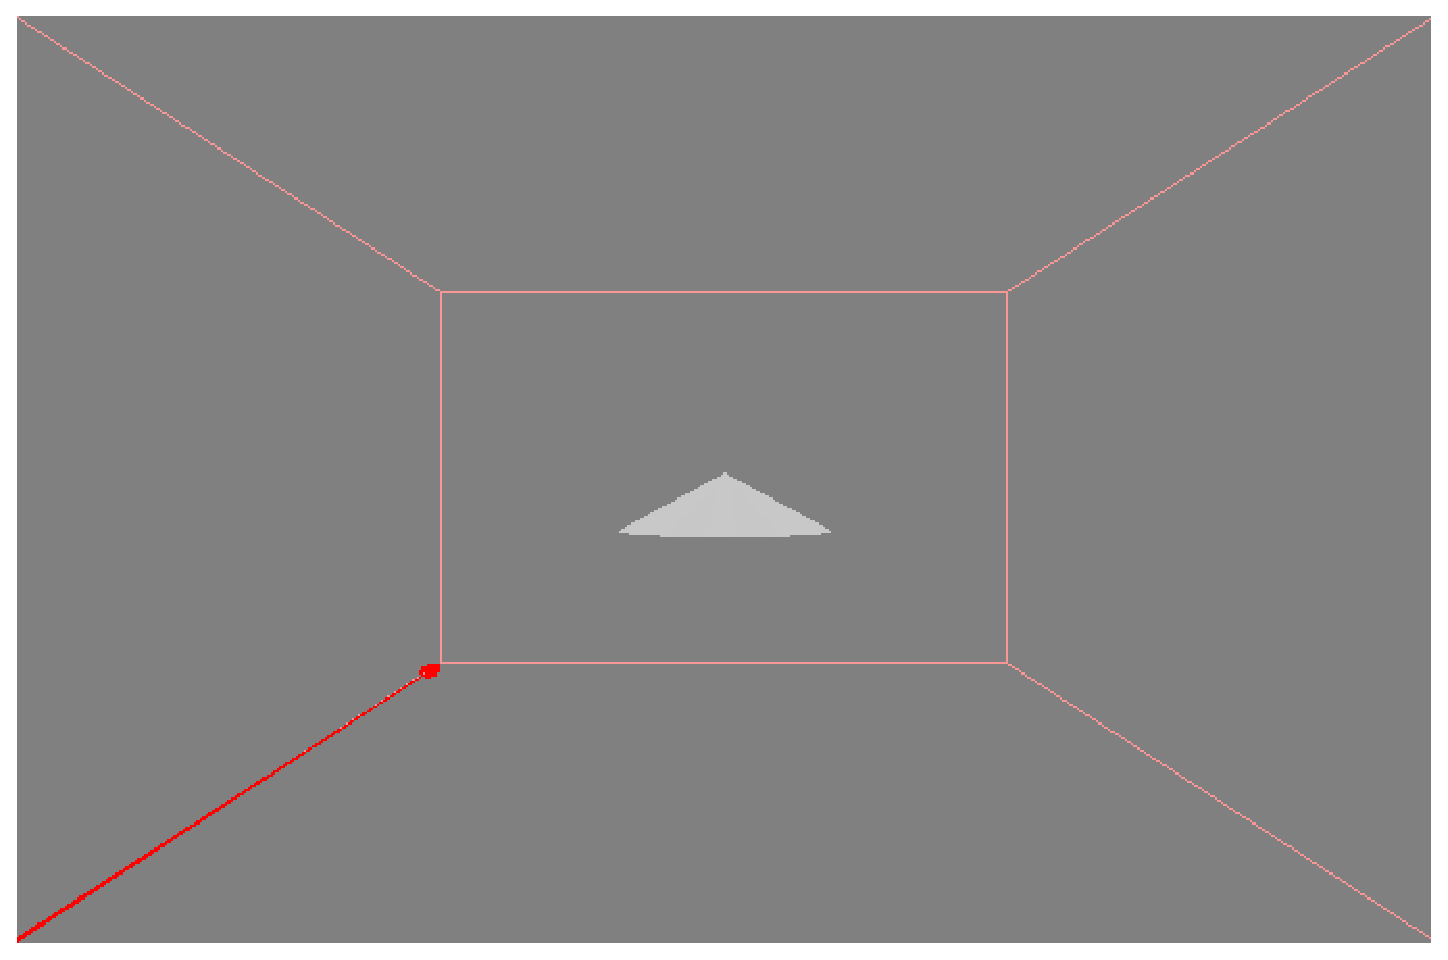
\includegraphics[scale = 0.4]{apr}
	\caption{Visualização de objeto por aproximação normal(sem mudança de foco).}
	\label{fg:apr}
\end{figure}
\begin{figure}[ht!]
	\centering
	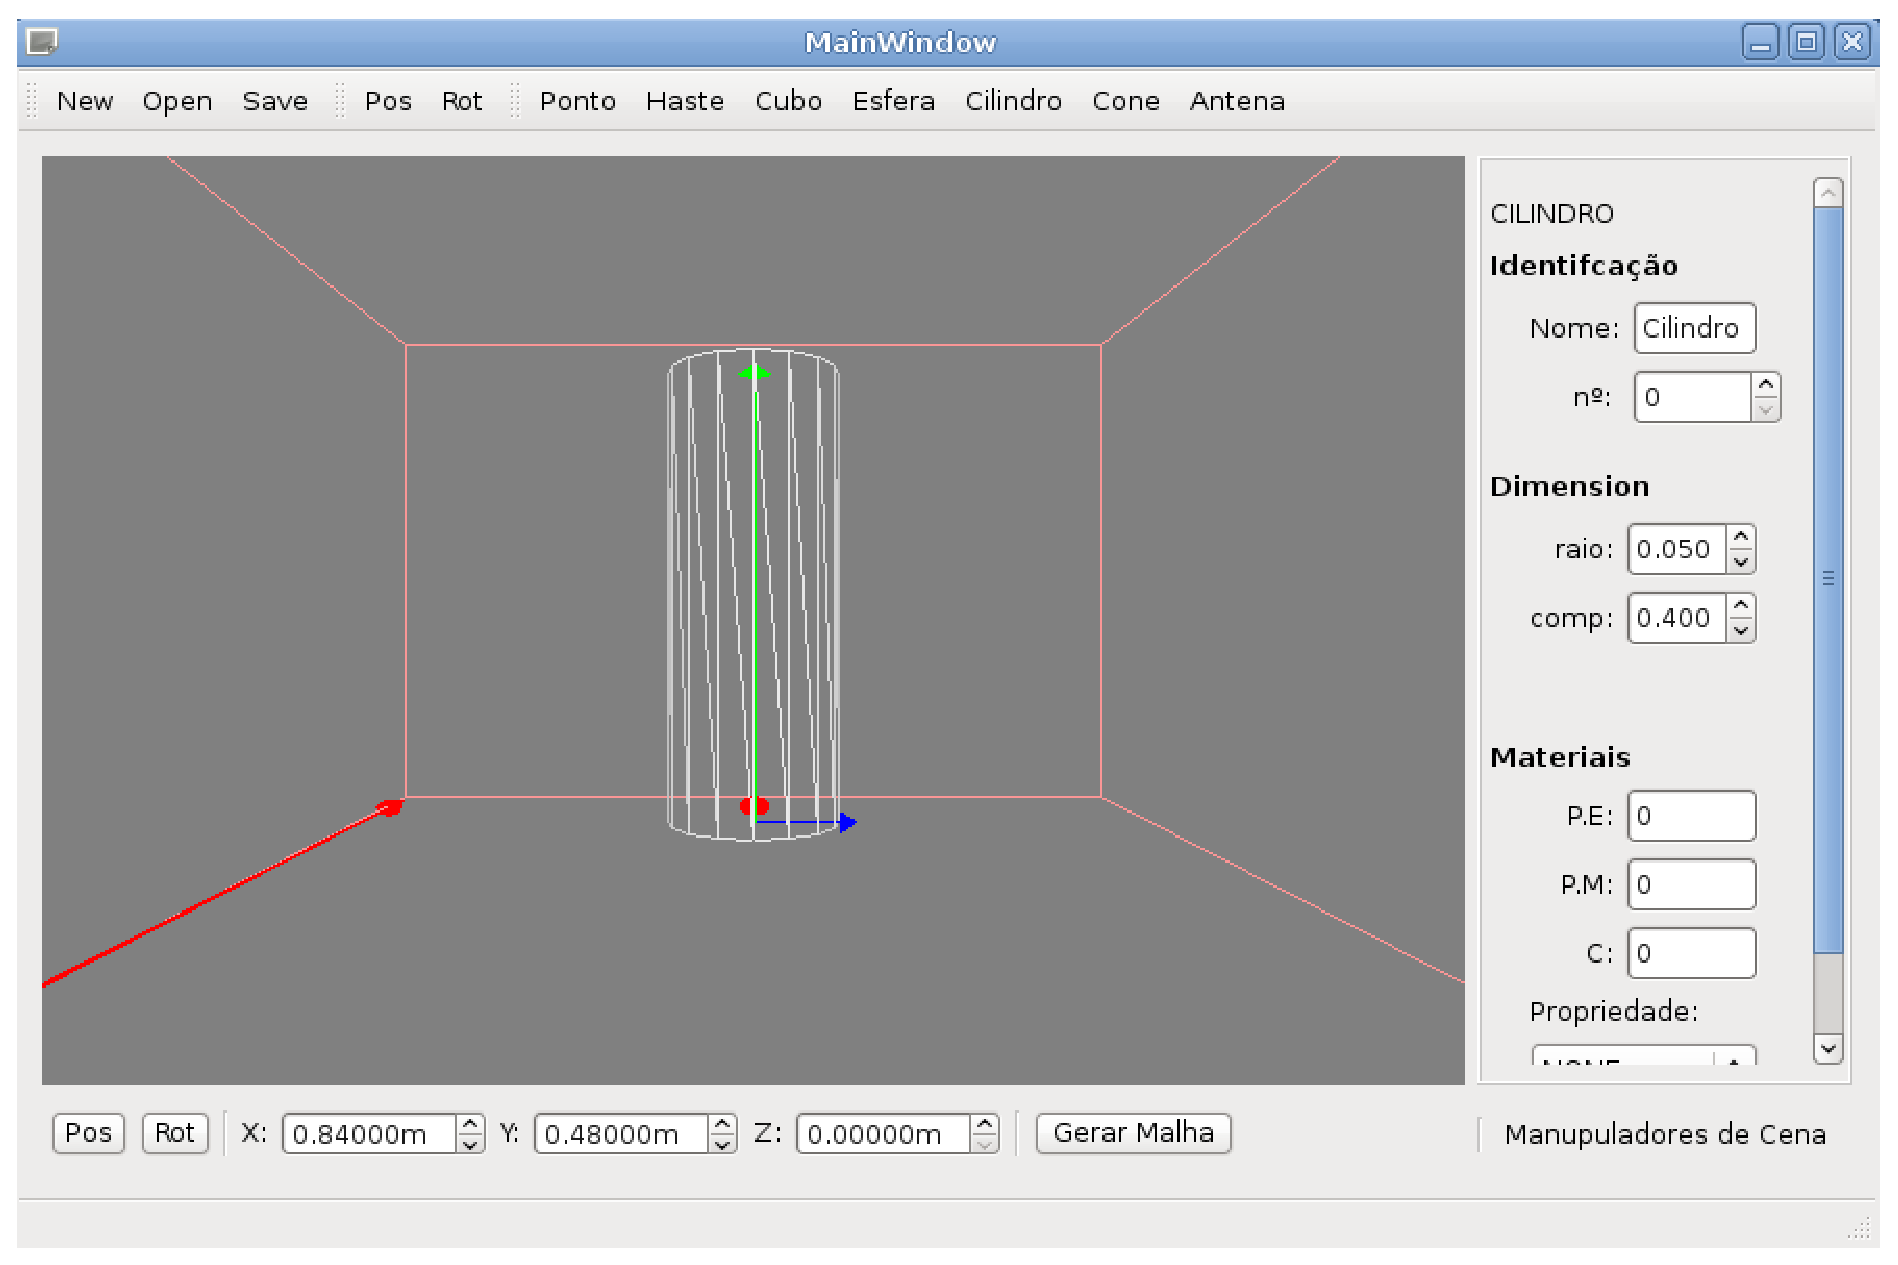
\includegraphics[scale = 0.4]{w}
	\caption{Focalização de objeto selecionado através do atalho de teclado W.}
	\label{fg:w}
\end{figure}

	\subsection{Remoção e Duplicação de Objetos}
	Nesse trabalho houve a necessidade criação de um mapa de objetos, pelo fato do irrlicht não permitir acesso ao seu array de objetos criados na cena. Dessa forma, qualquer alteração, remoção ou clonagem feita em um objeto na cena terá correspondência no mapa de \textit{nós} gerenciado pela interface. Com isso, quando removemos um objeto criado na região de análise, ele também será removido do mapa. As Figuras~\ref{fg:b_r} e \ref{fg:a_r} mostram a antes e depois de removermos um \textit{nó} do nosso universo virtual. \\
	
	O mesmo ocorre quando deseja-se duplicar um objeto, uma vez que isso ocorra o mapa receberá mais um \textit{nó} com as mesmas característica do selecionado. Esse evento esta representado pelas Figuras~\ref{fg:b_c} e \ref{fg:a_c}.
	
\begin{figure}[ht!]
	\centering
	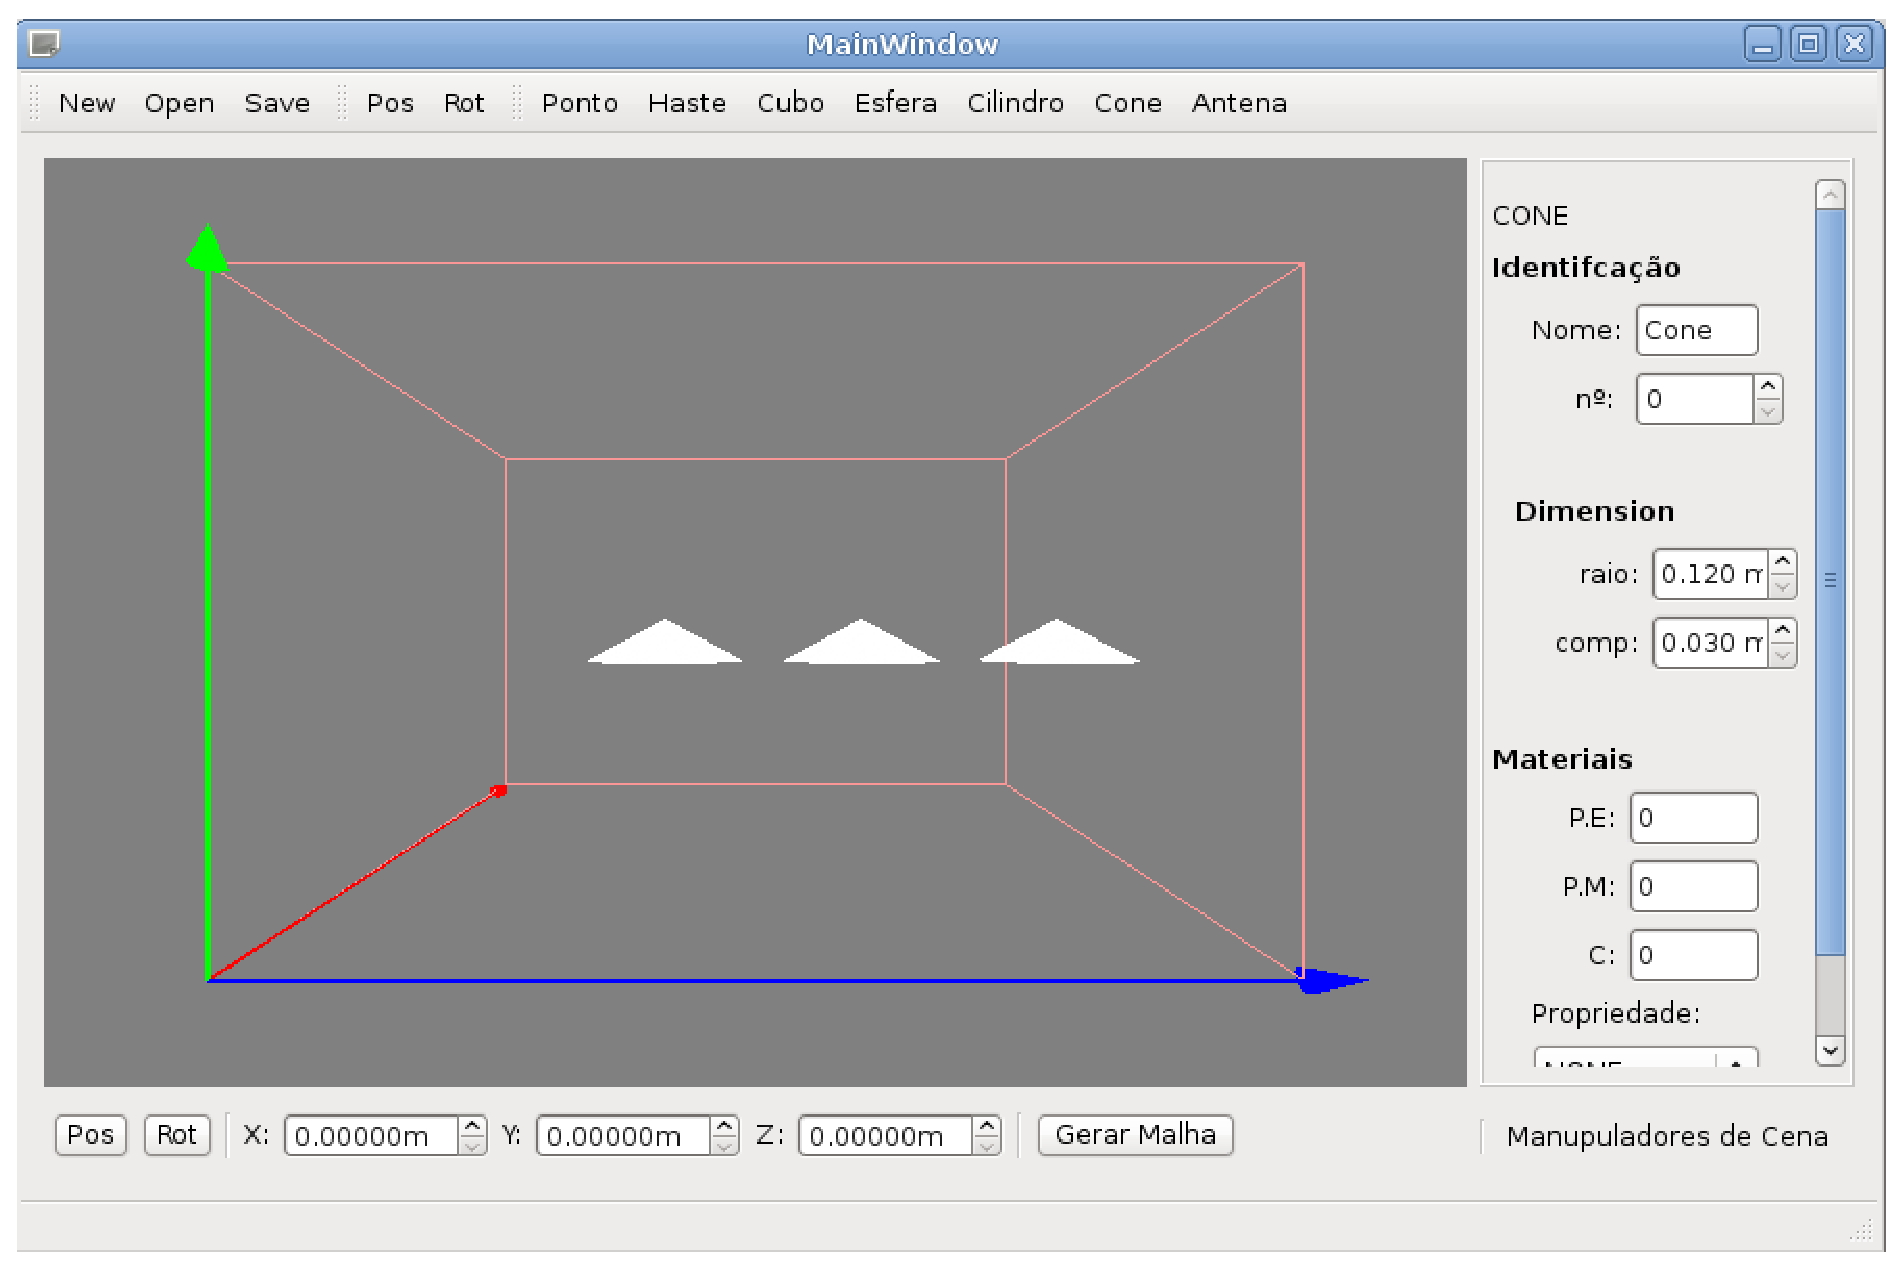
\includegraphics[scale = 0.4]{b_r}
	\caption{Antes da remoção.}
	\label{fg:b_r}
\end{figure}
\begin{figure}[ht!]
	\centering
	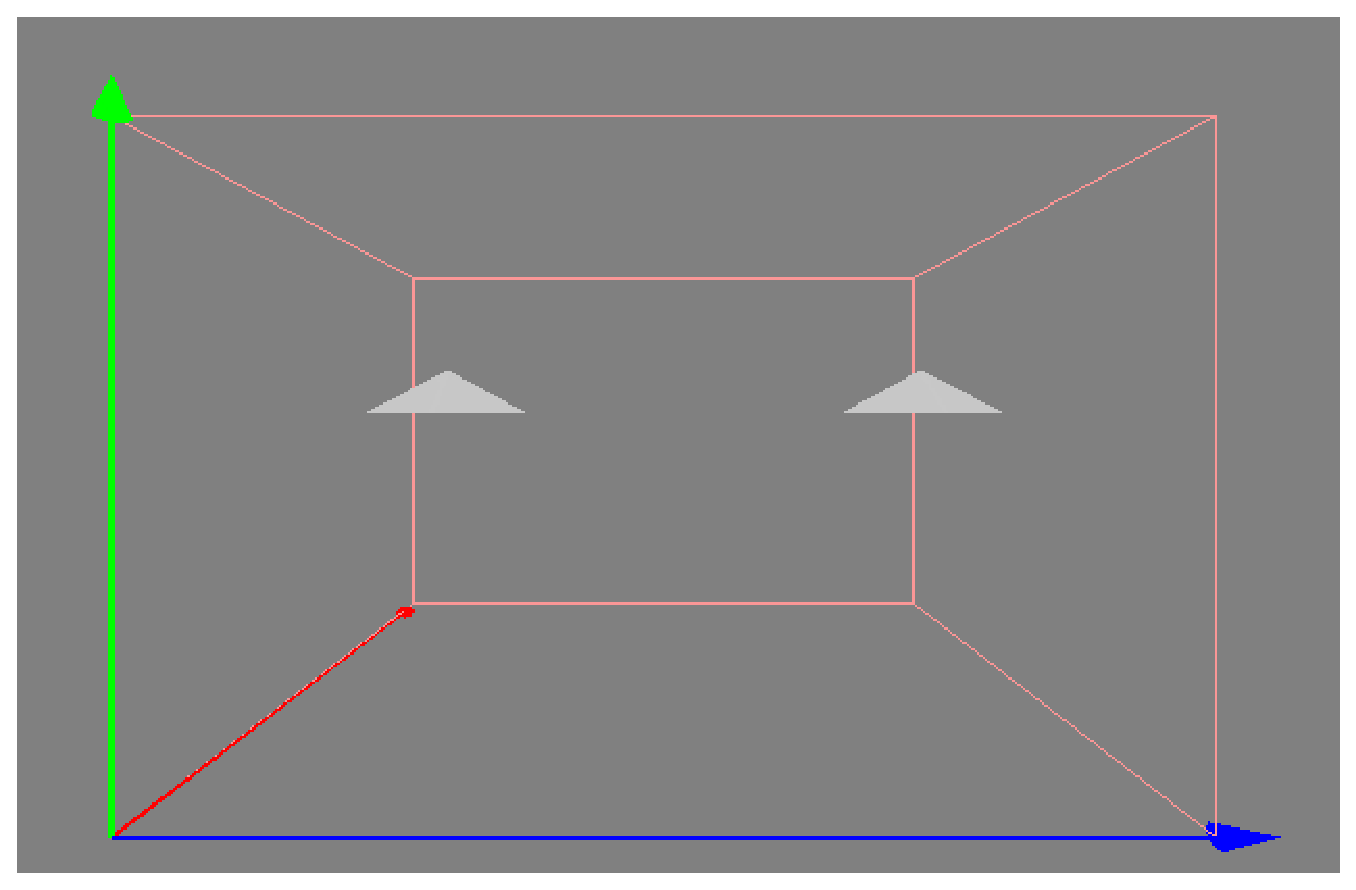
\includegraphics[scale = 0.4]{a_r}
	\caption{Depois da remoção.}
	\label{fg:a_r}
\end{figure}
\begin{figure}[ht!]
	\centering
	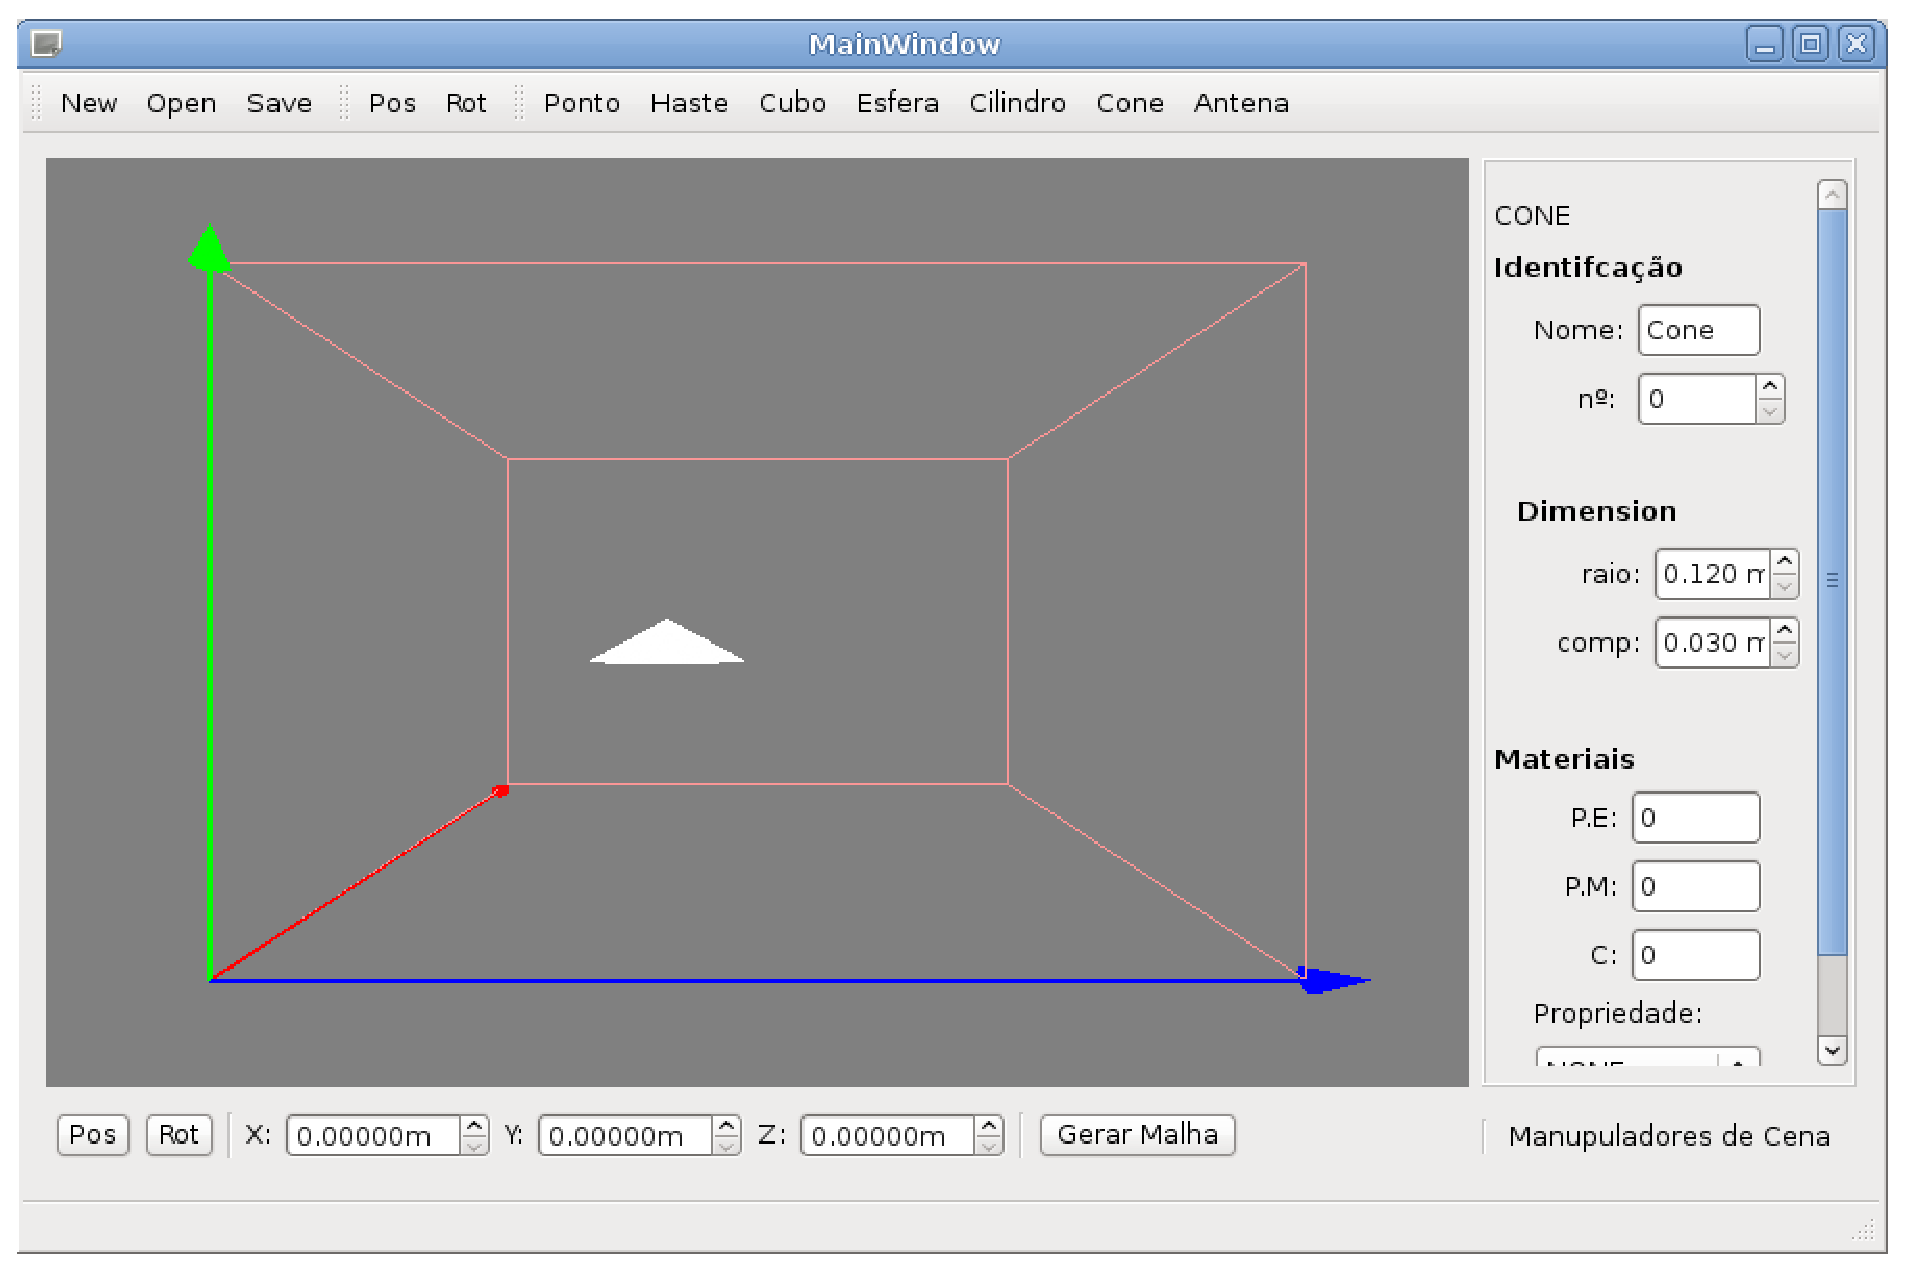
\includegraphics[scale = 0.4]{b_c}
	\caption{Antes da duplicação do objeto cone.}
	\label{fg:b_c}
\end{figure}
\begin{figure}[ht!]
	\centering
	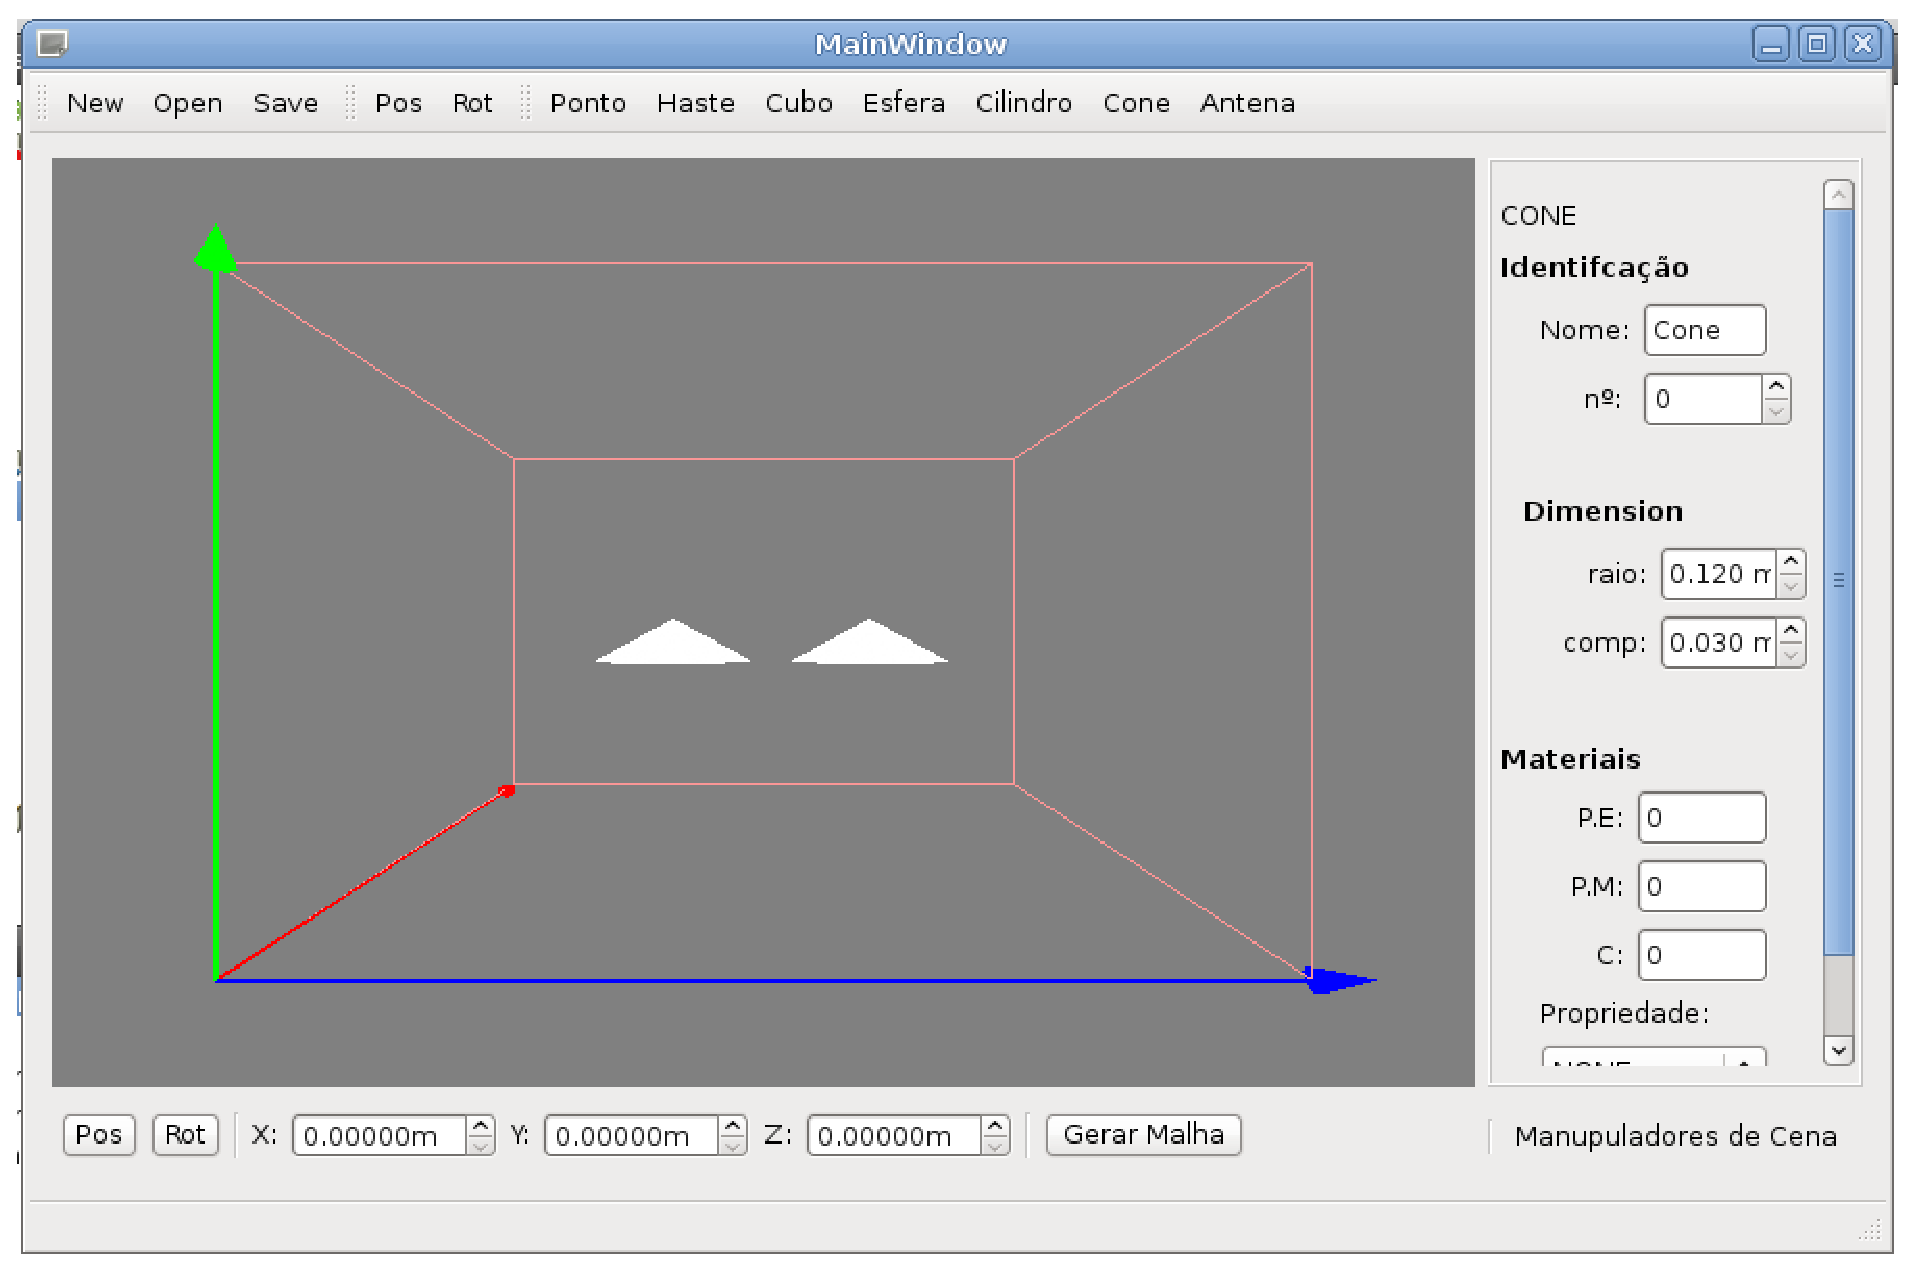
\includegraphics[scale = 0.4]{a_c}
	\caption{Depois da duplicação do objeto cone.}
	\label{fg:a_c}
\end{figure}

	\subsection{Conexão com o LANE-SAGS}
Como dito anteriormente a interface aqui produzida cria ambientes tridimensionais que podem ser utilizados em simulações em FDTD, porém, o mesmo não executa as simulações. Para que isso ocorra, é necessário o acoplamento desse ambiente com outro software que torne isso possível, o que é realizado através de arquivos de entrada e saída.\\
	
Esse software produzido nesse trabalho possui um sistema genérico de geração de arquivos de saída. Este sistema reconhece os objetos criados pela interface e cria uma representação destes objetos a partir de um conjunto de prismas retangulares. Cada prisma do conjunto representativo possui as características físicas de $\epsilon$(Permissividade Elétrica), $\sigma$(Condutividade Elétrica) e $\mu$(Permeabilidade Magnética) do objeto que representa.\\

A sequência de prismas representativos é gravada em um arquivo de saída chamado bd.in, compatível com o simulador LANE-SAGS. Cada prisma da sequência tem suas coordenadas e características físicas armazenados da seguinte forma: célula inicial $X$, célula final $X$, célula inicial $Y$, célula final $Y$, célula inicial $Z$, célula final $Z$,$\epsilon$, $\sigma$ e $\mu$; Além deste arquivo, contendo a sequência de prismas representativo dos objetos, é gerado um segundo arquivo chamado \textit{simconf.in} contendo as informações referentes às: dimensões das células de Yee (em metros) e a dimensão em células do Espaço Delimitador (região de análise).\\

Com a conexão realizado, basta adicionar alguns parâmetros como: antenas, planos de visualização, fonte, corrente; para então simular o ambiente. O diagrama mostrado na Figura \ref{fg:c_sags}, ilustra o processo de execução de uma simulação utilizando os dois softwares.
\begin{figure}[ht!]
	\centering
	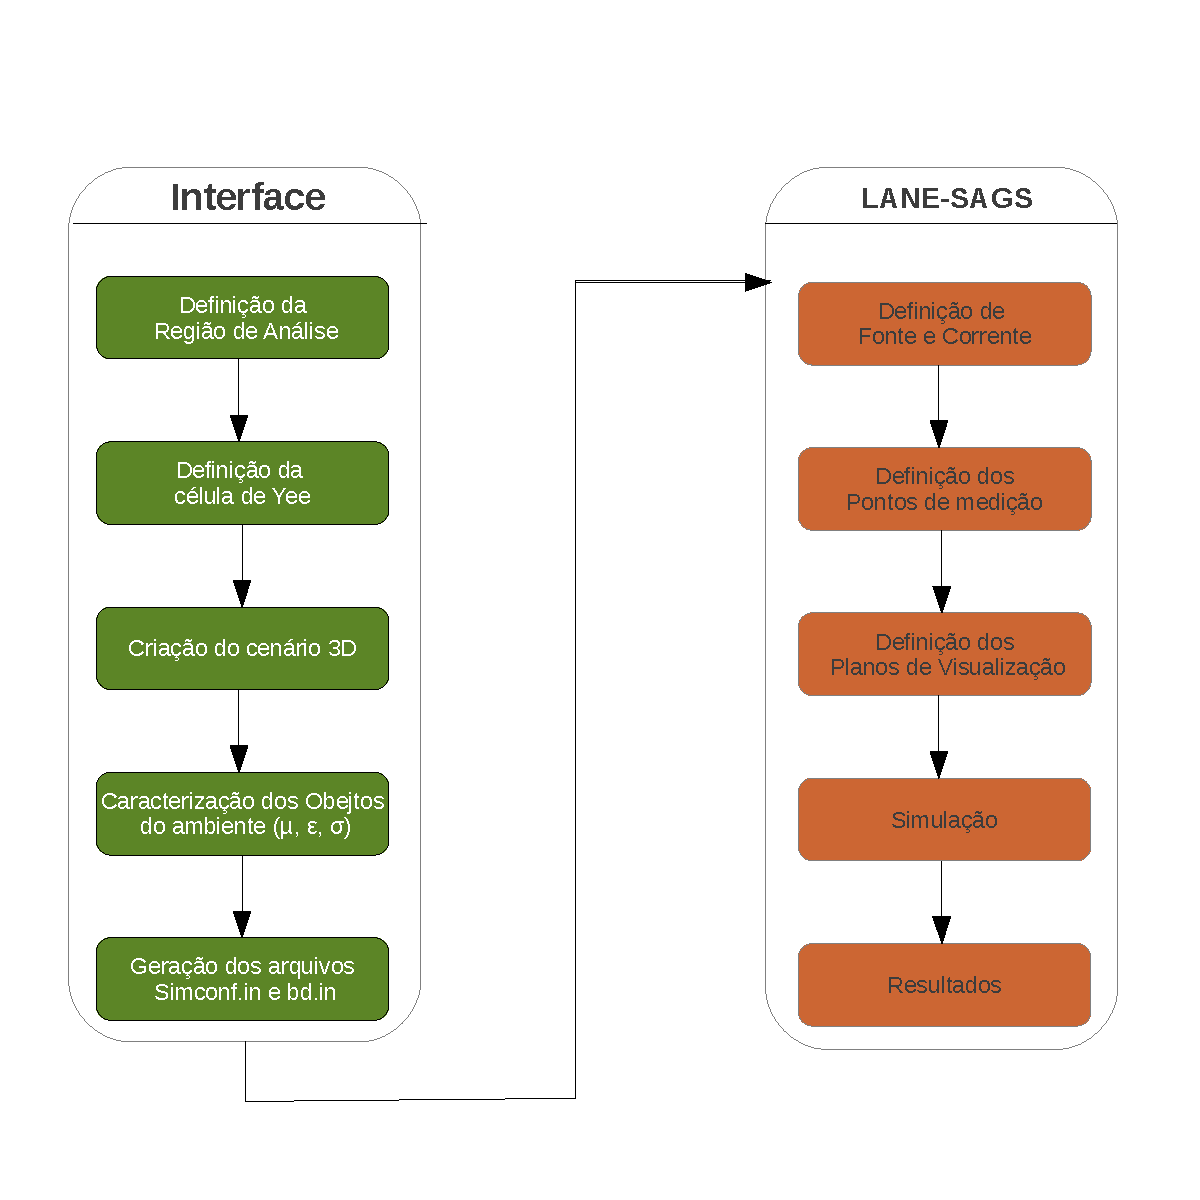
\includegraphics[scale = 0.4]{c_sags}
	\caption{Diagrama de conexão com o LANE-SAGS.}
	\label{fg:c_sags}
\end{figure}
